Let
%
\begin{align}
 XY=z,  YZ=x,  XZ=y
\end{align}
From the given information,
%
\begin{align}
y&= z\brak{\frac{\sin{Y}}{\sin{Z}}} 
&= 6 \brak{\frac{\sin{\ang{100}}}{\sin{\ang{50}}}}
&= 7.7134
\end{align}
and the vertices are
\begin{align}
\vec{X} &= \myvec{\ 0\\ 0}, \vec{Y} = z\myvec{ \cos X\si{\degree}\\ \sin X\si{\degree}} ,\vec{Z} =\myvec{y \\ 0} \\
\\
\implies \vec{X} &=\myvec{0 \\ 0},
\vec{Y} =6\myvec{\cos{\ang{30}} \\ \sin{\ang{30}}} &= \myvec{3\sqrt{3} \\ 3 }, 
\vec{Z} =\myvec{7.7134 \\ 0}
\end{align}
and plotted in Fig. \ref{july/2/3/Figure}.
%
\begin{figure}[!b]
  \centering
            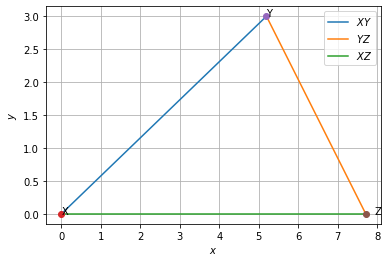
\includegraphics[width=\columnwidth]{solutions/july/2/3/Figure_1.png}
            \caption{Constructed Triangle}
            \label{july/2/3/Figure}
 \end{figure}
 %
 

